
\documentclass[12pt]{article}

\usepackage{sbc-template}
\usepackage{amsmath}

\usepackage{graphicx,url}

\usepackage[brazil]{babel}   
\usepackage[utf8]{inputenc}  
\usepackage{booktabs}
\usepackage[section]{placeins}
\usepackage{float}             



     
\sloppy

\title{Trabalho Pratico 1 - TCG}

\author{Arthur Henrique Tristão Pinto \inst{1}, Luis Henrique Ferreira Costa \inst{2}, Samuel Correia Pedrosa \inst{3} }


\address{Pontifícia Universidade Católica de Minas Gerais\\
 R. da Bahia, 2020 - Lourdes, Belo Horizonte - MG, 30160-012
}

\begin{document} 

\maketitle

\begin{abstract}
This work addresses the problem of identifying bridges in simple undirected graphs, which are edges whose removal disconnects the graph. Two distinct algorithms were implemented and analyzed for this purpose: a naïve method, which checks the graph's connectivity after removing each edge individually, and Tarjan's algorithm. Furthermore, both bridge-finding strategies were integrated into Fleury's algorithm to find Eulerian paths. The performance of these approaches was evaluated through computational experiments, measuring the average execution time on random graphs of varying orders (100, 1,000, 10,000, and 100,000 vertices) and classifications (Eulerian, semi-Eulerian, and non-Eulerian), allowing for a comparative analysis of the efficiency between the strategies.
\end{abstract}
     
\begin{resumo} 
  Este artigo descreve o problema da identificação de pontes em grafos simples não-direcionados, arestas cuja remoção desconecta o grafo. Foram implementados e analisados dois algoritmos distintos para esta finalidade: um método naïve, que verifica a conectividade do grafo após a remoção de cada aresta individualmente, e o algoritmo de Tarjan. Adicionalmente, as duas estratégias de detecção de pontes foram integradas ao algoritmo de Fleury para a busca de caminhos eulerianos. A avaliação de desempenho das abordagens foi realizada por meio de experimentos computacionais, medindo o tempo médio de execução em grafos aleatórios de diferentes ordens (100, 1.000, 10.000 e 100.000 vértices) e classificações (eulerianos, semi-eulerianos e não eulerianos), permitindo uma análise comparativa da eficiência entre as estratégias.
\end{resumo}

\newpage

\section{Contextualização} 

Algoritmos baseados em grafos são ferramentas fundamentais em diversas áreas da computação, auxiliando na resolução de inúmeros problemas complexos. Este trabalho se concentra em um problema específico da teoria dos grafos: a identificação de pontes em um grafo simples e não-direcionado.

\subsection{Estrutura do relatorio}

Este artigo está organizado em cinco seções principais. A primeira seção introduz o problema da identificação de pontes em grafos, estabelecendo os objetivos do trabalho. A segunda seção apresenta as definições formais de grafos, pontes e tipos de grafos(eulerianos,semi-eulerianos e não-eulerianos). A terceira seção detalha a metodologia empregada, incluindo o ambiente experimental, a geração dos grafos aleatórios e a implementação dos algoritmos propostos. A quarta seção analisa os resultados obtidos nos testes de desempenho. Finalmente, a quinta seção apresenta a conclusão do trabalho, sintetizando os resultados e as observações.

\section{Definições Formais}
\subsection{Grafos}

Um grafo simples n\~ao-direcionado, denotado por $G$, \'e formalmente definido como um par $G=(V,E)$. Nesse par:

\begin{itemize}
    \item $V$ representa o conjunto de v\'ertices.
    \item $E$ representa o conjunto de arestas.
\end{itemize}


\subsection{Pontes}

G=(V,E). Uma ponte é definida como uma aresta cuja remoção torna o grafo desconexo, ou seja, aumenta o número de componentes conectados. A capacidade de determinar as pontes existentes em um grafo é crucial para diversas aplicações, como na busca por caminhos e ciclos eulerianos.

\begin{figure}[ht]
\centering
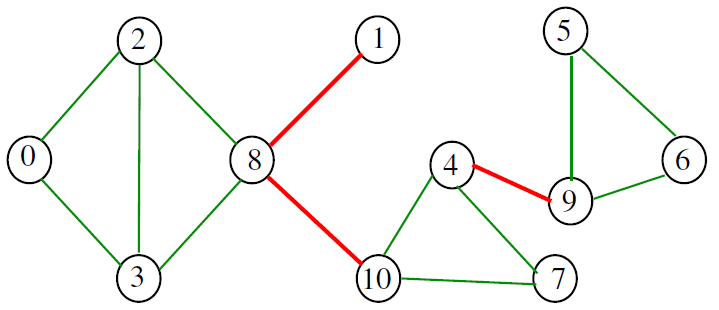
\includegraphics[width=.3\textwidth]{bridge.png}
\caption{Na figura, as arestas vermelhas são exemplos de pontes.}
\label{fig:exampleFig2}
\end{figure}

\subsection{Grafo Euleriano}
Um grafo $G$ \'e dito \textbf{euleriano} se ele possui um \textbf{ciclo euleriano} (ou \textbf{circuito euleriano}). Um ciclo euleriano \'e um caminho fechado que visita cada aresta do grafo exatamente uma vez, come\c{c}ando e terminando no mesmo v\'ertice.

\textbf{Condi\c{c}\~ao formal:} Um grafo conexo $G=(V,E)$ \'e euleriano se, e somente se, todo v\'ertice $v \in V$ possui \textbf{grau par}.
\begin{itemize}
    \item Matematicamente: $\forall v \in V, \text{deg}(v) \equiv 0 \pmod{2}$.
\end{itemize}

\begin{figure}[ht]
\centering
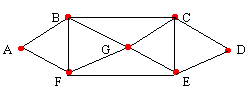
\includegraphics[width=.4\textwidth]{euleriano.png}
\caption{Exemplo de um grafo euleriano}
\label{fig:exampleFig3}
\end{figure}

\newpage

\subsection{Grafo Semi-Euleriano}
Um grafo $G$ \'e dito \textbf{semi-euleriano} se ele n\~ao possui um circuito euleriano, mas possui um \textbf{caminho euleriano}. Um caminho euleriano \'e um caminho aberto que visita cada aresta do grafo exatamente uma vez, come\c{c}ando e terminando em v\'ertices diferentes.

\begin{figure}[ht]
\centering
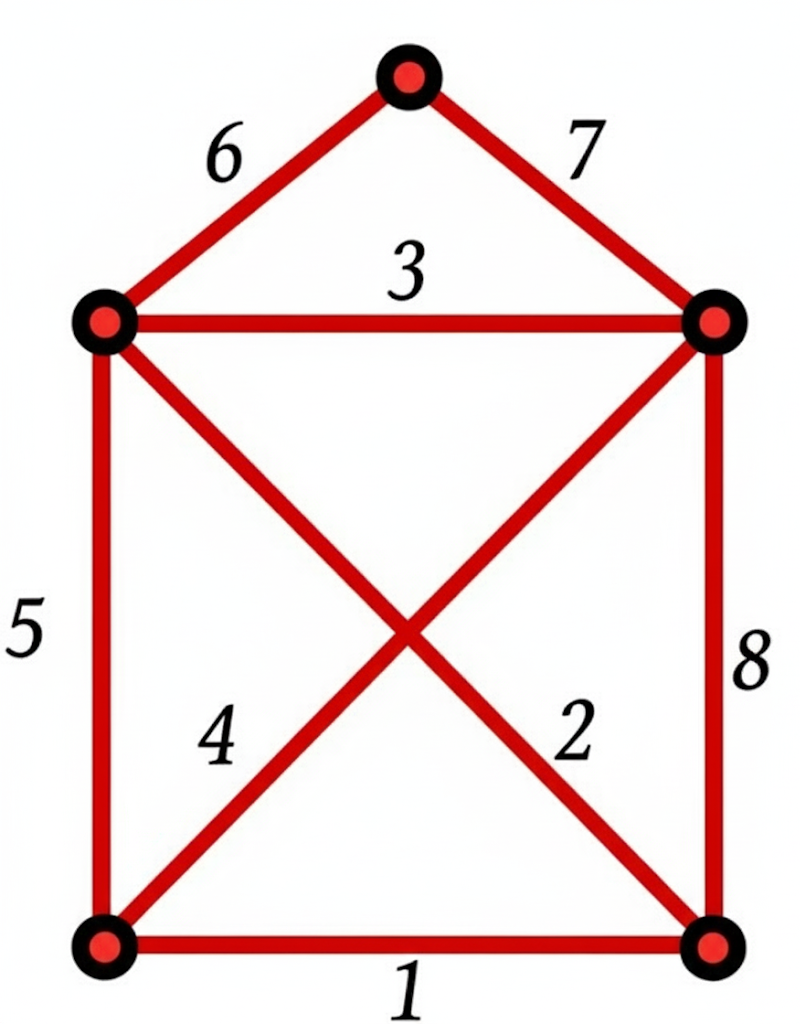
\includegraphics[width=.2\textwidth]{semi.png}
\caption{Exemplo de um grafo Semi-Euleriano}
\end{figure}

\subsection{Grafo N\~ao-Euleriano}
Um grafo $G$ \'e dito \textbf{n\~ao-euleriano} se ele n\~ao possui um caminho euleriano.


\textbf{Condi\c{c}\~ao formal:} Um grafo conexo $G=(V,E)$ \'e n\~ao-euleriano se, e somente se, ele possui \textbf{mais de dois v\'ertices de grau \'impar}.

\section{Metodologia}

\subsection{Ambiente e Ferramentas}

Para a implementação dos algoritmos e a condução dos experimentos, o ambiente de desenvolvimento foi composto pelo Java Development Kit (JDK) para compilação e execução do código-fonte. O desenvolvimento e a edição dos códigos foram realizados no editor Visual Studio Code, enquanto o versionamento e a colaboração no projeto foram gerenciados através da plataforma GitHub.

\subsection{Geração dos Grafos}

Para a avaliação experimental, foi desenvolvido um gerador de grafos em \textit{Java}
capaz de produzir instâncias aleatórias e conectadas, classificadas como
\textbf{eulerianas}, \textbf{semi-eulerianas} ou \textbf{não-eulerianas}.
O código do gerador baseia-se em três etapas principais:

\begin{enumerate}
    \item \textbf{Construção de um grafo base conexo.}\\
    Inicialmente é criado um \textit{grafo base}, garantindo que o grafo seja conectado
    e que todos os vértices possam ser alcançados em uma busca.
    Esse grafo contém $(N-1)$ arestas.
    Em seguida, são adicionadas arestas aleatórias até que o número total atinja o valor desejado $M$,
    evitando duplicatas e laços.
    
    \item \textbf{Cálculo dos graus dos vértices.}\\
    Após gerar a estrutura base, é calculado o grau de cada vértice. 
    A partir dessa informação, é possível identificar os vértices de grau ímpar
    e ajustar o grafo conforme o tipo desejado:
    \begin{itemize}
        \item \textbf{Euleriano:} todos os vértices devem ter grau par.
        Para isso, os vértices de grau ímpar são conectados em pares,
        tornando seus graus pares.
        \item \textbf{Semi-Euleriano:} exatamente dois vértices devem possuir grau ímpar.
        O gerador verifica a quantidade de ímpares e adiciona ou remove arestas
        de forma a manter apenas dois vértices ímpares.
        \item \textbf{Não-Euleriano:} o grafo deve possuir um número de vértices ímpares
        diferente de zero e de dois (no mínimo quatro ímpares).
        Quando necessário, o algoritmo força a criação de dois pares adicionais
        de vértices ímpares conectando vértices de grau par.
    \end{itemize}

    \item \textbf{Escrita em arquivo.}\\
    Por fim, o grafo é gravado em um arquivo texto contendo na primeira linha
    o número de vértices $N$, e nas linhas seguintes as arestas $(u, v)$.
    O formato é compatível com os programas implementados
    para execução dos algoritmos de Fleury.
\end{enumerate}

\subsection{Implementação dos Algoritmos de Identificação de Pontes}

A estratégia de busca para todas as implementações desenvolvidas neste artigo foi a busca em profundidade (DFS). A escolha desta abordagem foi diretamente inspirada pelo artigo de  \cite{Tarjan1972}

\subsubsection{Método Naive}

\begin{enumerate}
    \item \textbf{Teste de Conectividade (\texttt{buscaEmProfundidadeIterativaNaive}):}
    \begin{itemize}
        \item O m\'etodo central para verificar a conectividade \'e uma busca em profundidade (DFS) iterativa.
        \item A fun\c{c}\~ao percorre um componente do grafo e retorna o n\'umero total de v\'ertices que conseguiu alcan\c{car}. Este valor \'e usado como m\'etrica para determinar se o grafo permaneceu conectado.
    \end{itemize}

    \item \textbf{Algoritmo Principal (\texttt{pontesNaive}):}
    
    Esta fun\c{c}\~ao implementa o fluxo da abordagem Na\"ive, testando cada aresta.
    \begin{enumerate}
        \item \textbf{Linha de Base:} Primeiro, uma DFS \'e executada no grafo original para contar o n\'umero de v\'ertices alcan\c{c}\'aveis (\texttt{verticesEncontraveis}), que serve como refer\^encia.
        \item \textbf{Itera\c{c}\~ao sobre Arestas:} O algoritmo itera sobre uma lista de arestas \'unicas do grafo.
        \item \textbf{Processo "Remover-Testar-Restaurar":} Para cada aresta \texttt{(u, v)}, o ciclo \'e executado:
        \begin{itemize}
            \item \textbf{Remover:} A aresta \'e removida do grafo.
            \item \textbf{Testar:} Uma nova DFS conta os v\'ertices alcan\c{c}\'aveis (\texttt{alcancados}).
            \item \textbf{Comparar:} Se \texttt{alcancados < verticesEncontraveis}, a aresta \'e uma ponte.
            \item \textbf{Restaurar:} A aresta \'e adicionada de volta ao grafo.
        \end{itemize}
    \end{enumerate}
    Ao final, a fun\c{c}\~ao retorna a lista de todas as pontes encontradas.
    
    \item \textbf{Fluxo de Execu\c{c}\~ao (\texttt{main}):}
    \begin{itemize}
        \item O m\'etodo \texttt{main} gerencia a execu\c{c}\~ao: l\^e o grafo, invoca a fun\c{c}\~ao \texttt{pontesNaive} e imprime os resultados.
    \end{itemize}
\end{enumerate}

\subsubsection{Metodo Tarjan}

Metodo feito baseado no artigo de \cite{Tarjan1974}

\begin{enumerate}
    \item \textbf{Estruturas de Dados e Inicializa\c{c}\~ao:}
    \begin{itemize}
        \item \textbf{Grafo:} Representado por uma lista de adjac\^encias (\texttt{ArrayList<Integer>[]}).
        \item \textbf{Tabela de Busca (\texttt{TabelaBusca}):} Classe que armazena os metadados da busca para cada v\'ertice, contendo \texttt{TD} (Tempo de Descoberta), \texttt{TT} (Tempo de T\'ermino), \texttt{pai} e \texttt{low} (\textit{low-link}).
    \end{itemize}

    \item \textbf{Algoritmo Principal (\texttt{buscaEmProfundidadeIterativaTarjan}):}
    \begin{itemize}
        \item \textbf{Travessia DFS Iterativa:} A fun\c{c}\~ao inicia uma busca em profundidade a partir de um v\'ertice \texttt{vInicial}, controlada por uma \texttt{Stack} e iteradores.
        \begin{itemize}
            \item \textbf{Aresta de \'Arvore:} Ao encontrar um v\'ertice n\~ao visitado, seus valores \texttt{TD} e \texttt{low} s\~ao definidos e ele \'e empilhado.
            \item \textbf{Aresta de Retorno:} Se uma aresta leva a um v\'ertice j\'a visitado (que n\~ao seja o pai), o valor \texttt{low} do v\'ertice atual \'e atualizado com o \texttt{TD} do vizinho.
            \item \textbf{Propaga\c{c}\~ao do \texttt{low}:} Ao finalizar a an\'alise de um v\'ertice, seu valor \texttt{low} \'e propagado para seu pai na \'arvore DFS.
        \end{itemize}
        \item \textbf{Verifica\c{c}\~ao da Ponte:} Ap\'os a conclus\~ao da DFS, a fun\c{c}\~ao utiliza os valores calculados para verificar se a aresta \texttt{(v1, v2)}, fornecida como par\^ametro, satisfaz a condi\c{c}\~ao de ponte de Tarjan: \texttt{tabela[v2].low > tabela[v1].TD} (assumindo que \texttt{v1} \'e o pai de \texttt{v2}).
    \end{itemize}

    \item \textbf{Fluxo de Execu\c{c}\~ao (\texttt{main}):}
    \begin{itemize}
        \item O m\'etodo \texttt{main} l\^e o grafo, inicializa as estruturas e invoca a fun\c{c}\~ao de busca para analisar uma aresta espec\'ifica.
    \end{itemize}
\end{enumerate}

\subsection{Implementação de Fleury }

\subsubsection{Fleury com Naive}

\begin{enumerate}
    \item \textbf{Verifica\c{c}\~ao da Pr\'e-condi\c{c}\~ao Euleriana:}
    \begin{itemize}
        \item O algoritmo valida se o grafo possui no m\'aximo dois v\'ertices de grau \'impar, condi\c{c}\~ao necess\'aria para a exist\^encia de um caminho euleriano.
    \end{itemize}

    \item \textbf{Inicializa\c{c}\~ao:}
    \begin{itemize}
        \item Uma c\'opia do grafo original \'e criada para permitir a remo\c{c}\~ao de arestas sem alterar a entrada.
        \item Um v\'ertice inicial apropriado \'e selecionado (um de grau \'impar, se houver) e o caminho \'e iniciado.
    \end{itemize}

    \item \textbf{Constru\c{c}\~ao Iterativa do Caminho:}
    \begin{itemize}
        \item Um la\c{c}o \'e executado enquanto houver arestas. A escolha da pr\'oxima aresta \'e governada pela regra de Fleury, com a verifica\c{c}\~ao de pontes realizada pelo m\'etodo \texttt{ehPonteNaive}:
        \begin{itemize}
            \item \textbf{M\'etodo de Verifica\c{c}\~ao:} Para cada aresta candidata, a fun\c{c}\~ao \texttt{ehPonteNaive} a remove temporariamente e executa uma busca em profundidade (DFS) para contar o n\'umero de v\'ertices alcan\c{c}\'aveis. Se essa contagem for menor que a do grafo com a aresta, ela \'e uma ponte.
            \item \textbf{Sele\c{c}\~ao:} O algoritmo escolhe a primeira aresta que, segundo o teste, \textbf{n\~ao} \'e uma ponte. Se todas as op\c{c}\~oes forem pontes, a primeira da lista \'e selecionada.
        \end{itemize}
    \end{itemize}
    
    \item \textbf{Atualiza\c{c}\~ao e Conclus\~ao:}
    \begin{itemize}
        \item A aresta escolhida \'e permanentemente removida da c\'opia do grafo, o novo v\'ertice \'e adicionado ao caminho e a posi\c{c}\~ao atual \'e atualizada. O processo se repete at\'e que todas as arestas sejam consumidas.
    \end{itemize}
\end{enumerate}

\subsubsection{Fleury com Tarjan}

\begin{enumerate}
    \item \textbf{Verifica\c{c}\~ao da Pr\'e-condi\c{c}\~ao Euleriana:}
    \begin{itemize}
        \item O algoritmo primeiramente verifica se o grafo possui no m\'aximo dois v\'ertices de grau \'impar. Caso contr\'ario, um caminho euleriano \'e imposs\'ivel e a execu\c{c}\~ao \'e interrompida.
    \end{itemize}

    \item \textbf{Inicializa\c{c}\~ao:}
    \begin{itemize}
        \item Uma c\'opia do grafo original (\texttt{G\_prime}) \'e criada para que as opera\c{c}\~oes de remo\c{c}\~ao de arestas n\~ao afetem a estrutura original.
        \item Um v\'ertice inicial \'e selecionado, priorizando um de grau \'impar, se existente. O caminho resultante \'e inicializado com este v\'ertice.
    \end{itemize}

    \item \textbf{Constru\c{c}\~ao Iterativa do Caminho:}
    \begin{itemize}
        \item Um la\c{c}o \'e executado enquanto houver arestas no grafo-c\'opia. A cada passo, a partir do v\'ertice atual \texttt{v\_atual}, a pr\'oxima aresta \'e escolhida seguindo a regra de Fleury:
        \begin{itemize}
            \item \textbf{Caso 1 (Aresta \'Unica):} Se h\'a apenas uma aresta dispon\'ivel, ela \'e selecionada.
            \item \textbf{Caso 2 (M\'ultiplas Arestas):} O algoritmo testa cada aresta candidata com a fun\c{c}\~ao \texttt{buscaEmProfundidadeIterativaTarjan}. A primeira aresta que \textbf{n\~ao} for uma ponte \'e escolhida. Se todas forem pontes, a primeira da lista \'e selecionada como \'ultimo recurso.
        \end{itemize}
    \end{itemize}
    
    \item \textbf{Atualiza\c{c}\~ao e Conclus\~ao:}
    \begin{itemize}
        \item Ap\'os a escolha, a aresta \'e removida do grafo-c\'opia, o novo v\'ertice \'e adicionado ao caminho e a posi\c{c}\~ao atual \'e atualizada.
        \item O processo se repete at\'e que todas as arestas sejam percorridas. Ao final, a fun\c{c}\~ao retorna a lista de v\'ertices que comp\~oem o caminho euleriano.
    \end{itemize}
\end{enumerate}

\section{Testes}

\subsection{Estratégia de Avaliação}
Nesta seção são apresentados os resultados experimentais obtidos na execução dos algoritmos
\textit{Fleury\_Naive} e \textit{Fleury\_Tarjan}.
Os testes foram realizados em grafos com diferentes números de vértices
($N = 100$, $1\,000$, $10\,000$ e $100\,000$), cada um tendo aproximadamente em média N*1.5 número de arestas
com o objetivo de comparar o tempo de execução entre as duas abordagens.

Para cada valor de $N$, foram gerados e testados \textbf{12 grafos distintos}:
\textbf{4 eulerianos}, \textbf{4 não-eulerianos} e \textbf{4 semi-eulerianos}.
Os tempos médios e os desvios padrão apresentados a seguir correspondem à média dos resultados
obtidos nesses 12 grafos, medidos em milissegundos.
\subsection{Resultados Quantitativos}
\begin{table}[h!]
\centering
\caption{Tempo médio e desvio padrão (em milissegundos) para os algoritmos \textit{Fleury\_Naive} e \textit{Fleury\_Tarjan}.}
\label{tab:tempos}
\begin{tabular}{l r r r}
\toprule
\textbf{Algoritmo} & \textbf{Vértices} & \textbf{Média (ms)} & \textbf{Desv. Padrão (ms)} \\
\midrule
Fleury\_Naive  & 100       & 10.50   & 9.58   \\
Fleury\_Naive  & 1\,000    & 108.08  & 82.3   \\
Fleury\_Naive  & 10\,000   & 8\,008.17 & 5\,873.81  \\
Fleury\_Naive  & 100\,000  & 1\,400\,803.83 & 1\,051\,130.70 \\
\midrule
Fleury\_Tarjan & 100       & 9.58    & 8.62   \\
Fleury\_Tarjan & 1\,000    & 80.25   & 68.2   \\
Fleury\_Tarjan & 10\,000   & 3\,923.42  & 3\,043.51\\
Fleury\_Tarjan & 100\,000  & 770\,652.58 & 596\,471.87  \\
\bottomrule
\end{tabular}
\end{table}

\subsection{Visualização dos Resultados}

\begin{figure}[H]
    \centering
    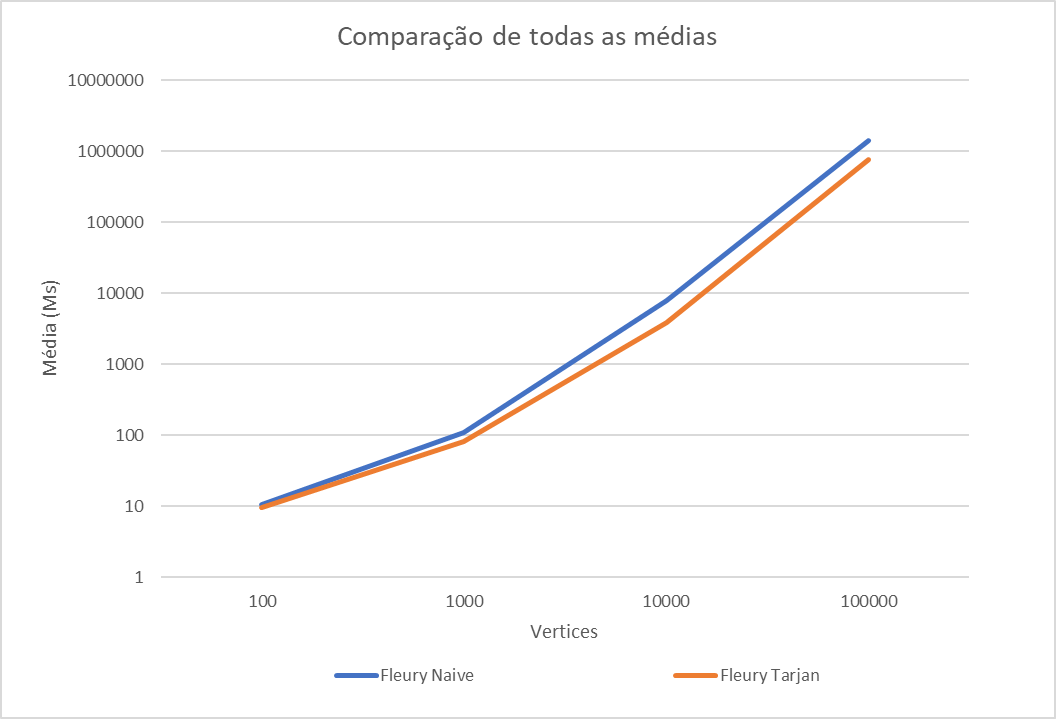
\includegraphics[width=0.8\textwidth]{grafico_geral.png}
    \caption{Crescimento do tempo médio de execução (ms) conforme o número de vértices.}
    \label{fig:grafico_geral}
\end{figure}

\subsubsection{Comparação para N = 100}
% --- MUDANÇA AQUI ---
\begin{figure}[H]
    \centering
    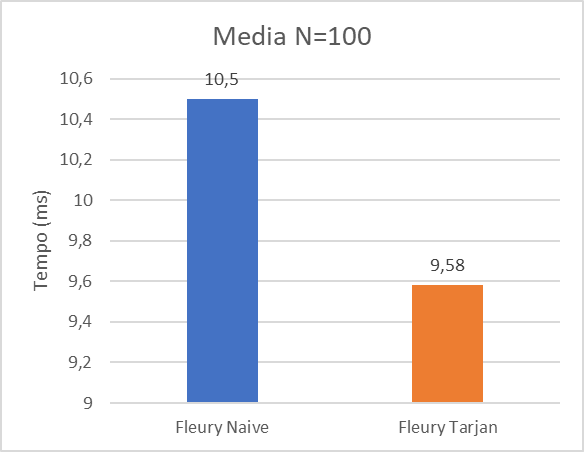
\includegraphics[width=0.6\textwidth]{grafico_100.png}
    \caption{Comparação da média de tempo entre os algoritmos para $N = 100$.}
    \label{fig:grafico_100}
\end{figure}

\subsubsection{Comparação para N = 1\,000}
% --- MUDANÇA AQUI ---
\begin{figure}[H]
    \centering
    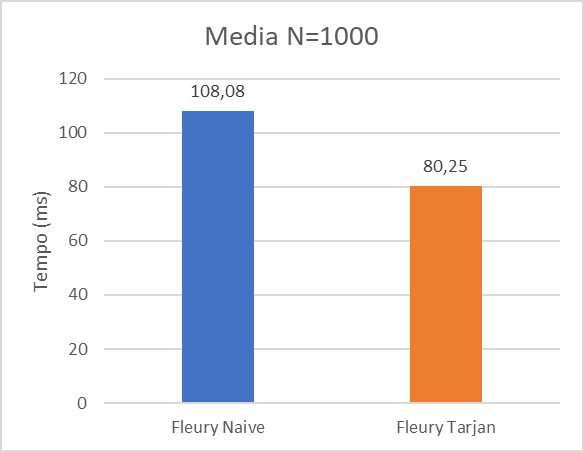
\includegraphics[width=0.6\textwidth]{grafico_1000.png}
    \caption{Comparação da média de tempo entre os algoritmos para $N = 1\,000$.}
    \label{fig:grafico_1000}
\end{figure}

\subsubsection{Comparação para N = 10\,000}
% --- MUDANÇA AQUI ---
\begin{figure}[H]
    \centering
    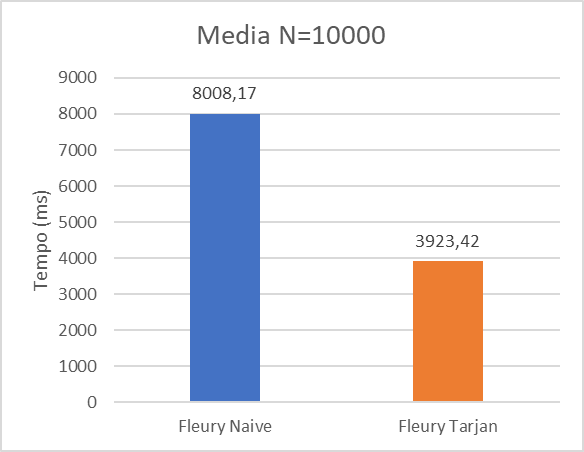
\includegraphics[width=0.6\textwidth]{grafico_10000.png}
    \caption{Comparação da média de tempo entre os algoritmos para $N = 10\,000$.}
    \label{fig:grafico_10000}
\end{figure}

\subsubsection{Comparação para N = 100\,000}
% --- MUDANÇA AQUI ---
\begin{figure}[H]
    \centering
    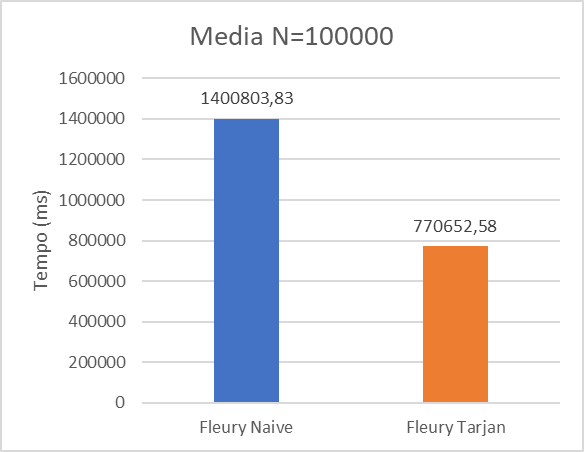
\includegraphics[width=0.6\textwidth]{grafico_100000.png}
    \caption{Comparação da média de tempo entre os algoritmos para $N = 100\,000$.}
    \label{fig:grafico_100000}
\end{figure}

\section{Discussão de Resultados}

Após os testes realizados, observa-se que o algoritmo \textbf{Fleury\_Tarjan} apresenta desempenho consistentemente superior ao \textbf{Fleury\_Naive}, especialmente à medida que o número de vértices dos grafos aumenta.

Para grafos pequenos (100 vértices), a implementação \textbf{Fleury\_Tarjan} (9,58~ms) já se mostra ligeiramente mais eficiente que a \textbf{Fleury\_Naive} (10,50~ms). No entanto, à medida que o número de vértices cresce, a vantagem do algoritmo otimizado com Tarjan torna-se significativamente mais evidente. Para 10~000 vértices, a versão com Tarjan (3~923~ms) é cerca de duas vezes mais rápida que a Naive (8~008~ms). O cenário mais expressivo ocorre com 100~000 vértices, em que o \textbf{Fleury\_Tarjan} (770~652~ms) executa em aproximadamente metade do tempo do \textbf{Fleury\_Naive} (1~400~804~ms), confirmando sua melhor escalabilidade.

Os altos desvios-padrão observados resultam das diferenças estruturais entre os grafos \textit{eulerianos}, \textit{semi-eulerianos} e \textit{não eulerianos}, que demandam quantidades distintas de verificações e travessias. Essa variação reflete a diversidade de complexidade das instâncias testadas, e não uma inconsistência dos algoritmos.



\bibliographystyle{sbc}
\bibliography{sbc-template}

\end{document}

